\documentclass[twocolumn, linenumbers, superscriptaddress, nofootinbib]{revtex4-1}

\usepackage{amsmath}
\usepackage{graphicx}
\usepackage{gensymb}
\usepackage{textgreek}
\usepackage{xcolor}
\usepackage{microtype}
\usepackage[colorlinks]{hyperref}
	\hypersetup{colorlinks,
	linkcolor={red!50!black},
	citecolor={blue!60!black},
	urlcolor={blue!40!black}
	}
\graphicspath{{figures/}}
%-------------------------------------------------------------------------------

\begin{document}
	\begin{abstract}
		The acorn weevil (\textit{Curculio} Linnaeus, 1758) rostrum (snout) exhibits remarkable flexibility and toughness derived from the microarchitecture of its exoskeleton.
		Here we characterize modifications to the composite profile of the rostral cuticle that simultaneously enhance the flexibility and toughness of the distal portion of the snout.
		Using Classical Laminate Plate Theory, we estimate the effect of these modifications on the elastic behavior of the exoskeleton.
		We show that the tensile behavior of the rostrum across six \textit{Curculio} species with high morphological variation correlates with changes in the relative layer thicknesses and orientation angles of layers in the exoskeleton.
		Accordingly, increased endocuticle thickness is strongly correlated with increased tensile strength.
		Rostrum stiffness is shown to be inversely correlated with work of fracture; thus allowing a highly curved rostrum to completely straighten without structural damage.
		Finally, we identify exocuticle rich invaginations of the occipital sutures both as a likely site of crack initiation in tensile failure, and as a source of morphological constraint on the evolution of the rostrum in \textit{Curculio} weevils.
	\end{abstract}
	
	%title and author block
	{\title{Exoskeletal strength and cuticle composite profile of the acorn weevil rostrum}
	\date{\today}
	
	\author{M. Andrew Jansen}
		\email[corresponding author, email:~]{majanse1@asu.edu}
		\affiliation{School of Life Sciences, Arizona State University, Tempe, AZ 85287, USA}
	\author{Jason Williams}
		\affiliation{School for Engineering of Matter, Energy, and Transport, Arizona State University, Tempe, AZ 85287, USA}
	\author{Nikhilesh Chawla}
		\affiliation{School for Engineering of Matter, Energy, and Transport, Arizona State University, Tempe, AZ 85287, USA}
	\author{Nico M. Franz}
		\affiliation{School of Life Sciences, Arizona State University, Tempe, AZ 85287, USA}
		
	\maketitle
	}

	The exoskeleton of Coleoptera (beetles) is a hierarchically structured, fibrous composite -- characterized by variously arranged \textalpha-chitin (N-acetylglucosamine) nanofibrils that are embedded in a heterogeneous protein matrix \cite{Hepburn1973, Jansen2016, Vincent2004}.
	Although \textalpha-chitin is brittle and strongly anisotropic, beetle cuticle is simultaneously rigid and tough due to its unique laminate microstructure (reviewed in \cite{Kamp2010, Kamp2015, Neville1976}), characterized in detail below.
	Impact-prone areas and exaggerated structures in arthropods generally exhibit cuticle organization that resists deformation and fracture \cite{Amini2015, Mccullough2014mech, Mccullough2014struc, Dirks2012, Dirks2013}.
	However, acorn weevils in the genus \textit{Curculio} Linnaeus, 1758\footnote{
		Pursuant to the International Code of Zoological Nomenclature, the first mention of any specific epithet will include the full genus and species names as a binomen (two-part name) followed by the author and date of publication of the name.
		This is not an in-line reference; it is a part of the name itself and refers to a particular act establishing the validity and fixing the identity of the corresponding name by that author \cite{ICZN1999}.}
	(Curculionidae in the sense of \cite{Davis2014}) instead exhibit unusual distal flexibility in an elongate extension of the head called the rostrum (snout) \cite{Toju2005, Jansen2016, Singh2016, Gibson1969}.
	The rostrum is a hollow, strongly curved (over 90$\degree$ in some species), cylindrical, exoskeletal extension of the otherwise nearly-spherical head, which bears at its apex the terminal chewing mouthparts \cite{Morimoto2003, Ting1933, Ting1936, Dennell1942, Gibson1969}.
	This structure is used by the female to feed on fruit (plant) tissue and to excavate sites for egg-laying (oviposition, see Fig.~\ref{fig::curculio}).
	The rostrum can be repeatedly bent, without evident damage, and despite being composed of the same material as other rigid body parts \cite{Jansen2016, Singh2016, Gibson1969, Toju2005}.
	By maintaining constant pressure on the snout and rotating around the bore-hole, females are able to flex the rostrum into a straightened configuration and produce a linear channel into the fruit.
	A single adult female may prepare hundreds of such sites \cite{Toju2005, Moffett1989, AguirreUribe1978}.
	
	\begin{figure*}
		\centering
		\includegraphics[width=180mm]{fig1.pdf}
		\caption{\textbf{Morphology and oviposition behavior of female \textit{Curculio} weevils.} 
			\textbf{a}, Lateral habitus image of female \textit{Curculio~sayi} (Gyllenhal, 1836) featuring the elongate, strongly curved rostrum.
			\textbf{b}, Lateral view of head of female specimen of \textit{Curculio~longinasus} Chittenden, 1927, with major anatomical features indicated.
			\textbf{c}, Illustration of oviposition behavior, proceeding from left to right: female makes incision in host fruit, flexes head directly over bore-hole using front legs, then maintains tension on snout while rotating to excavate linear channel into fruit. During this process, female rostrum is bent until completely straight.
		}
		\label{fig::curculio}
	\end{figure*}
	
	Despite its documented performance in many \textit{Curculio} species \cite{Gibson1969, Moffett1989, AguirreUribe1978, Toju2005}, it remains unknown how the rostrum of female acorn weevils can withstand the repeated, often extreme bending incurred during the process of egg-chamber excavation.
	In this study, we therefore characterize the composite profile of the rostral cuticle to account for the observed flexibility of the snout.
	We show that the relative layer thicknesses and fiber orientation angles of the exocuticle and endocuticle of the rostrum are strongly differentiated from the head capsule and other body parts.
	The effect of these differences on the elasticity of the cuticle is estimated using Classical Laminate Plate Theory (CLPT).
	Recent studies have shown that the yield strength of the beetle exoskeleton is lower in tension than compression \cite{Longhai2017}.
	To assess the validity of these findings, we compare the ultimate tensile strength of the rostrum across species and snout morphotypes.
	We also report displacement-controlled load cycling results for the snout of one \textit{Curculio} species with strongly curved morphology.
	Our results indicate that an increase in the volume fraction of endocuticle in the rostrum conveys higher tensile strength at the rostral apex across all tested species; and further, that a strongly curved rostrum can be flexed repeatedly without harm to the structure.
	
	We additionally describe the fracture mechanics of the snout, while considering how modification of the cuticle may prevent crack formation during oviposition.
	Accordingly, the flexibility and tensile strength of the rostrum appear to be derived \emph{exclusively} from modification of the composite architecture of the exoskeleton.
	This is the first time that a modified composite profile has been reported as a means of enhancing structural elasticity in the insect exoskeleton (though see \cite{Matsumura2017}).
	
	
	\section{Microstructure of the \textit{Curculio} rostrum}
		In arthropods -- including beetles - the exocuticle is comprised of numerous unidirectional laminae of chitin nanofibrils.
		Each layer is the thickness of a single fiber (2-4 \,nm) embedded in a proteinaceous matrix \cite{Nikolov2010, Nikolov2011}.
		These layers are stacked at a more or less constant angle to each other, forming a quasi-isotropic laminate known as the Bouligand structure \cite{Blackwell1980, Bouligand1972, Neville1976}. 
		This layout effectively mitigates the strong anisotropy of \textalpha-chitin, thus yielding a versatile building material for the exoskeleton \cite{Vincent1982, Vincent2004, Nikolov2010, Nikolov2011}.		
		Beetle endocuticle, however, is unique among arthropods and is comprised of large -- 1-5 \,{\textmu}m diameter in \textit{Curculio} -- unidirectional bundles of chitin, called macrofibers.
		Chitin macrofibers are orthotropic (axial: $E_1~=~8.5~\,\text{GPa}$; transverse: $ E_2~=~E_3~=~0.52~\,\text{GPa}$ \cite{Jansen2016}), and arranged in unidirectional plies, as depicted in Figs.~\ref{fig::cuticle},~\ref{fig::profile} \cite{Kamp2010, Kamp2015}.
		Typically, adjacent macrofiber laminae are paired and pseudo-orthogonal -- i.e., angled nearly $90\degree$ to each other (see Fig.~\ref{fig::profile}; \cite{Cheng2009}) -- with a constant stacking angle \emph{between} pairs, although other configurations have been observed \cite{Hepburn1973, Kamp2010, Kamp2015, Leopold1992}.
		This geometric sequence of the macrofiber laminae yields an approximately transversely isotropic composite, similar to the Bouligand structure \cite{Kamp2015, Nikolov2010}.
		Notably, the resulting laminate is less rigid than the exocuticle, but exhibits greater toughness because the pseudo-orthogonal plies effectively inhibit crack formation and propagation between successive layers \cite{Kamp2010, Kamp2015, Hepburn1973}.
		
		\begin{figure*}
			\centering
			\includegraphics[width=180mm]{fig2.pdf}
			\caption{\textbf{Gross divisions of cuticle in the female \textit{Curculio} rostrum.}
				\textbf{a}, Scanning electron micrograph of head capsule, in frontal view, of female \textit{Curculio~sulcatulus} (Casey, 1897), with rostrum removed.
				\textbf{b}, Magnified view of junction between rostrum and head capsule, showing division of cuticle into two general regions: exocuticle and endocuticle.
			}
			\label{fig::cuticle}
		\end{figure*}
		
		Serial thin sectioning and scanning electron microscopy of fractured \textit{Curculio} specimens reveals that endocuticle in the head capsule fits this general profile, with an angle of nearly $30\degree$ between successive pairs of pseudo-orthogonal plies.
		Additionally, in the head capsule, the thickness of the exocuticle and endocuticle in cross-section is nearly equal -- typically between 20-30 \,{\textmu}m.
		However, the cuticle composite lay-up of the rostral apex is strongly differentiated from the head capsule, as shown in Fig.~\ref{fig::profile}.
		Distally the exocuticle is reduced to a thin shell (ca. 5 \,{\textmu}m), with the endocuticle thickened to offset this reduction and maintain a constant cuticle thickness (ca. 50 \,{\textmu}m total) throughout its length.
		Moreover, the endocuticular macrofibers exhibit no rotation between successive pseudo-orthogonal plies; and are oriented at approximately $\pm45\degree$ to the longitudinal axis of the snout (i.e., an antisymmetric $[\pm45\degree]$ angle-ply laminate).
		We previously identified these modifications to the composite structure of the cuticle within a single species, \textit{Curculio longinasus} Chittenden, 1927 \cite{Jansen2016, Singh2016}.
		However, this composite profile is herein reported in the rostrum of six additional, phylogenetically disjoint, species, suggesting that this is an evolutionarily conserved trait throughout the genus \textit{Curculio}.
		In all examined species, the portion of the snout between the head capsule and apex of the scrobe exhibits a gradual transition in composite profile along an anterior-posterior gradient.
		
		\begin{figure*}
			\centering
			\includegraphics[width=180mm]{fig3.pdf}
			\caption{\textbf{Composite profiles of rostral \textit{Curculio} cuticle.}
				\textbf{a}, Scanning electron micrograph of fractured specimen of \textit{Curculio~humeralis} (Casey, 1897), showing that cuticle of rostral apex is organized as $\pm45\degree$ angle-ply laminate.
				\textbf{b}, Scanning electron micrograph of fractured specimen of \textit{Curculio~caryae} (Horn, 1873), showing that cuticle of rostral base and head capsule has approximately $30\degree$ stacking angle between each pair of pseudo-orthogonal plies.
				\textbf{c--d}, Semi-thin sections of cuticle from specimen of \textit{Curculio humeralis}, stained with toluidine-blue-borax; demonstrating:
				(\textbf{c}) that exocuticle of rostral apex is reduced to thin shell close to 5\,{\textmu}m thick, with endocuticle thickened to maintain a constant laminate thickness; and, 
				(\textbf{d}) that exocuticle of head capsule and base of snout occupies nearly half of through-thickness of cuticle.
			}
			\label{fig::profile}
		\end{figure*}
		
		Here we estimate the effect of differential cuticle organization on uni-axial membrane and on transverse-flexural Young's moduli of the cuticle in the rostral apex and head capsule using CLPT \cite{Reddy2004, Jones2014}.
		The effective elastic constants of the cuticle regions of \textit{Curculio longinasus} -- estimated previously \cite{Jansen2016} -- are used to construct constitutive equations for the entire cuticle of that species.
		The cuticle of the head capsule is estimated to have membrane and flexural moduli of $E_m~=~4.77~\,\text{GPa}$ and $E_f~=~6.04~\,\text{GPa}$, respectively.
		In the rostral apex these values are reduced by approximately 72\% and 60\%, respectively ($E_m~=~1.36~\,\text{GPa}; E_f~=~2.44~\,\text{GPa}$).
		Two hypothetical cuticle lay-ups are also modeled to individually assess the contributions of either modified layer thickness or stacking angle sequence to the cuticle's flexibility.
		The effective moduli of a configuration with the angle stacking sequence of an otherwise typical cuticle (i.e., in the head capsule) that shows layer thicknesses of the rostral apex are calculated as $E_m~=~3.73~\,\text{GPa}, E_f~=~4.31~\,\text{GPa}$; representing 22\% and 29\% decreases from unmodified cuticle, respectively.
		Similarly, a hypothetical cuticle with the layer thicknesses of ordinary cuticle yet possessing the angle stacking sequence of the rostral apex (i.e., $\pm45\degree$ angle-ply in the endocuticle) has effective elastic moduli of $E_m~=~3.77~\,\text{GPa}, E_f~=~5.76~\,\text{GPa}$; representing 21\% and 4.7\% decreases from unmodified cuticle, respectively.
		Each of the cuticle modifications noted in the rostral apex individually decrease the elastic moduli of the cuticle.
		However, they appear to have a synergistic combined effect on cuticle elasticity, rather than a simple additive effect.
		This result suggests that both modifications are necessary in order for the snout to function properly in the living individual -- where the combined effect allows the rostrum to bend until completely straight without fracture.
	
	\section{Force-controlled loading to fracture}
		
		\begin{figure*}
			\centering
			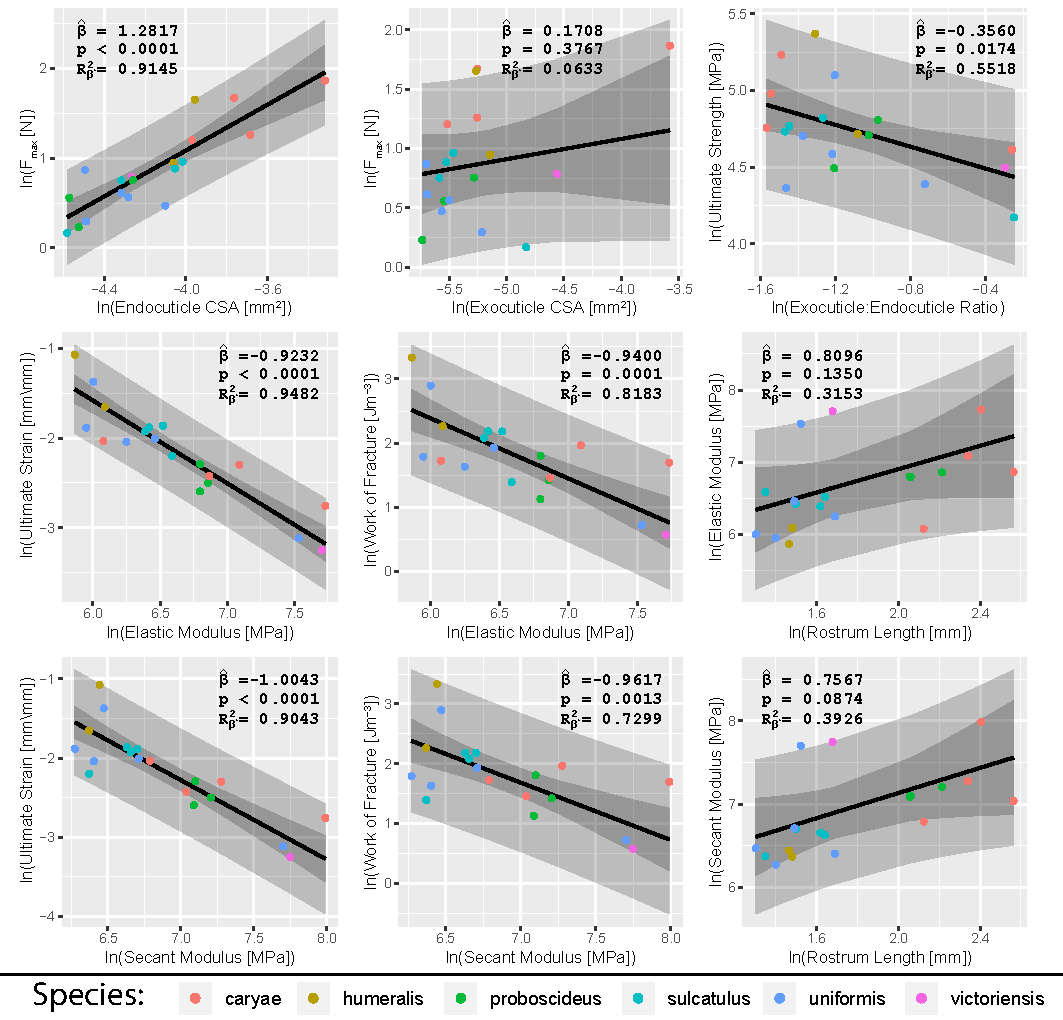
\includegraphics[width=180mm]{fig4.pdf}
			\caption{\textbf{Tensile properties of the female \textit{Curculio} rostrum.}
				Each plot shows relationship between two variables as predicted by phylogenetic linear mixed-effect model; with species as random effect and variance-covariance matrix generated from Brownian motion over preferred phylogeny of \cite{Bonal2016}.
				Gray regions represent the prediction interval and bootstrapped 95\% confidence interval of model.
				The estimated fixed effect $\hat{\beta}$ is given, along with p-value of t-test assessing whether $\hat{\beta}$ is significantly different from zero.
				Generalized marginal $\text{R}^2_{\beta^*}$ for assessing fixed effects is also reported.
				In general, increased endocuticle thickness is associated with greater tensile strength, and stiffness is inversely correlated with toughness.
			}
			\label{fig::tensile}
		\end{figure*}		
	
		To better characterize the failure behavior of the female rostrum, we performed tensile testing on the snouts of six \textit{Curculio} species that representing a mixture of closely and distantly related taxa \cite{Hughes2004phylo, Hughes2004eco, Bonal2016, Bonal2011}.
		Each specimen was first immersed in $\text{di-H}_2\text{O}$ for 24 hours to simulate the living tissue (see \cite{Klocke2011}), then subjected to force-controlled, uniaxial loading to fracture at a constant stress rate of $1.0\,\text{gf}\cdot\text{s}^{-1}$.
		In general, the specimens exhibited a non-linear viscoelastic response curve characterized by a sharp increase in stress at higher strains, terminating in brittle fracture \cite{Mihai2017}.
		We suggest that strain hardening occurs as the longitudinal axis of the macrofibers becomes more closely aligned to the cylindrical axis of the rostrum, thereby resisting tension more directly with increasing strain \cite{Munster2013}.
			
		We also examined the correspondence between composite structure and mechanical behavior of the snout in an evolutionary, comparative context.
		Phylogenetic linear mixed effects models (PGLM, Fig.~\ref{fig::tensile}) were used to account for phylogenetic non-independence in residual variance, with species membership included as a random effect \cite{Revell2010, Felsenstein1985}.
		The resulting models show that the maximum force sustained at the site of failure is strongly correlated with the cross-sectional area of the endocuticle ($\hat{\beta}=1.28,~p<0.0001$), and not the exocuticle ($\hat{\beta}=0.17,~p=0.38$), at that site.
		There is thus a negative correlation between ultimate tensile strength of the specimen and the cross-sectional exocuticle-to-endocuticle area ratio at the fracture site ($\hat{\beta}=-0.36,~p=0.017$).
		Although CLPT predicts a positive association between the proportion of exocuticle and stiffness of a generalized cuticle, we found no evidence of correspondence between the cross-sectional properties of the fracture site and the overall performance of the rostrum.
		This result is not too surprising however; because the cross-sectional areas of the cuticle regions vary across the length of the head along an anterior-posterior gradient, it is not possible to correlate measurements from the fracture surface to properties of the entire rostrum.
		
		Instead, we found that the uniaxial elastic modulus (low strain: $E_{low}$) and secant modulus at failure ($E_{sec}$) were inversely correlated with ultimate strain and work of fracture (see Fig.~\ref{fig::tensile}).
		This implies that stiffer specimens -- and by extension, stiffer cuticle profiles -- are generally more brittle.
		We also observed a moderate, but not statistically significant, stiffening size-effect with respect to rostral length.
		This runs contrary to our expectation that a longer, more strongly curved rostrum would require increased flexibility to avoid fracture during oviposition \cite{Hughes2004eco, Bonal2011}.
		It is possible that longer rostra also have a longer transition gradient from basal to apical profile; thereby reinforcing the junction between the rostrum and head capsule against buckling.
		Young's modulus of the rostrum would be comparatively higher in such species, due to the higher volume fraction of exocuticle.
		We therefore posit that the gross elastic performance of the cuticle is consistent across the weevil genus \textit{Curculio}.
		A \emph{single} mechanism -- i.e., the modified composite profile -- likely confers increased flexibility and tensile strength to the rostral apex across all \textit{Curculio} species.
		In addition, the endocuticle demonstrably contributes more to rostral tensile strength than the exocuticle; likely because of its organization into large bundles of aligned, anisotropic fibers, and amounting a trade-off between rigidity and toughness.
		Consequently, the altered composite profile of the cuticle in the rostral apex makes the rostrum simultaneously more flexible and fracture-resistant.
		
	\section{Load cycling of the pecan weevil}
		
		\begin{figure*}
			\centering
			\includegraphics[width=180mm]{fig5.pdf}
			\caption{\textbf{Fatigue testing of a female \textit{Curculio caryae} rostrum.}
				\textbf{a}, Set-up of fatigue testing, with female's head capsule fixed to pedestal and rostrum attached to strip of rip-stop nylon fabric using cyanoacrylate adhesive.
				Specimen was loaded in tension, as opposed to compression, therefore isolating effect of tension on fatigue behavior of rostrum.
				\textbf{b}, Overlay of pre- and post-fatigue states of head, showing clear (short-term) effect from repeated prescribed strain.
				\textbf{c}, Three-photograph sequence of pre- and post-fatigue states of the rostrum; with left and central panels showing conditions immediately prior to and after testing, respectively, whereas right panel shows head having returned to its original shape after 24 hours off soaking in a water/ethanol mixture. Hence immediate post-fatigue shape is not permanent.
				\textbf{d}, Raw force data (left) and displacement data (right) plots for fatigue test.
				Displacement data plot shows clear viscoelastic behavior, indicated by histeresis in stress-strain response of specimen, and exhibits logarithmic decrease stress amplitude over time.
			}
			\label{fig::fatigue}
		\end{figure*}
		
		To confirm that repeated, prescribed straightening of the rostrum does not result in damage to the cuticle, we performed displacement-controlled fatigue testing on a typical female specimen of the pecan weevil \textit{Curculio caryae} (Horn, 1873) -- a species that exhibits extreme ($80-90\degree$, Fig.~\ref{fig::fatigue}) rostral curvature \cite{AguirreUribe1978, Gibson1969}.
		The specimen was aligned so that uniaxial tension would induce elongation of the distal portion of the rostrum with minimal off-axis deflection of the uncurved section.
		The strain per cycle was fixed at an amplitude sufficient to completely elongate the rostrum and generate a tensile load of 1.0\,N  in the straightened configuration (ca. 20\% ultimate strength), at a frequency of $0.33\,\text{Hz}$.
		The test was terminated after a period of two weeks -- i.e., ca. 400,000 cycles -- when the stress amplitude appeared to reach an asymptotic minimum.		
		The rostrum behaved viscoelastically, indicated by histeresis in the stress-strain relationship during each cycle.
		Strain amplitude decreased logarithmically with cycle number, and the specimen appeared to have been deformed plastically and permanently during the test.
		However, after cleaning the specimen in a 24-hour wash with ethanol and water, the rostrum had returned to its original shape (Fig.~\ref{fig::fatigue}).
		
		While we cannot fully determine the cause for rostrum stress relaxation \emph{after} testing, we speculate that it arose from the general mechanism associated with cuticle viscoelasticity.
		The endocuticle is made of aligned \textalpha-chitin nanofibrils whose crystalline structure is enforced by hydrogen bonds between individual chitin chains and through the protein matrix along their length.
		Macroscopic viscoelastic behavior results from slippage between these chains in response to shearing between the chitin molecules \cite{Vincent2004, Evans1967, Sun2012}.
		Repeated strain may have caused such slippage in the endocuticle of the rostral apex during the fatigue test
		Without sufficient time for the material to \textit{completely} relax after deformation, the rostrum would slowly accumulate strain and deform viscoelastically \cite{Munster2013}.
		After immersion in ethanol and water, however, the cuticle would be sufficiently plasticized to allow the rostrum to return to its original configuration, thus dissipating the accumulated strain.
		
		The specimen did not show any evidence of fractures, micro-tears, or shear cusps anywhere in the surface of the exocuticle.
		Moreover, the tensile strength of the tested specimen's rostrum was consistent with that of other species members ($F_{max}~=~5.02~\,\text{N}$).
		Surprisingly, the specimen remained undamaged by the testing.
		We therefore conclude that under normal life conditions, repeated bending of the rostrum does not exceed the yield strength of the cuticle.
			
	\section{Fractography of \textit{Curculio} test specimens}
		
		\begin{figure*}
			\centering
			\includegraphics[width=180mm]{fig6.pdf}
			\caption{\textbf{Fractography of female \textit{Curculio} rostrum.}
				\textbf{a}, Light micrograph showing the fracture surface of tensile tested \textit{Curculio caryae} rostrum, displaying typical failure mode; illustrated in (\textbf{b}):
				Small, black arrows indicate the winding direction of macrofiber lamina; green arrows and dotted lines indicate the direction of crack.
				Scanning electron micrographs highlight: (\textbf{c}) shear cusp formation; (\textbf{d}) tensile failure and off-axis macrofiber fiber-pulling; (\textbf{e}) interlaminar delamination; (\textbf{f}-\textbf{h}) crack formation near invaginated exocuticle; and (\textbf{g}) ventral crack-front coalescence and shear cusp formation.
			}
			\label{fig::fracture}
		\end{figure*}
		
		In light of the complex failure modes evident in the fractured specimens, it was not always possible to identify void nucleation and crack initiation sites.
		We observed several patterns characteristic of both the micro-scale behavior of the cuticle and the meso-scale behavior of the rostrum during uniaxial tensile failure (Fig.~\ref{fig::fracture}).
		These patterns are described below.
		
		In transverse view, the exocuticle consistently presented a nearly continuous fracture surface.
		This is characteristic of comparatively brittle failure -- presumably due to the relatively homogeneous arrangement of \textalpha-chitin laminae in the Bouligand structure \cite{Nikolov2010, Nikolov2011}.
		The exocuticle typically appeared to fracture at lower strains than the endocuticle, with shear-cusp formation evident both at the fracture surface and across exocuticle adjacent to the plane of fracture \cite{Greenhalgh2009}.
		Conversely, the endocuticle exhibited severe delamination, off-axis ply-splitting, and fiber-pulling away from the fracture surface.
		This is indicative of the relatively high toughness of the unidirectional \textalpha-chitin organization within the macrofibers \cite{Kamp2010, Kamp2015}.
		Because the exocuticle of weevils is anchored to the endocuticle by cross-linking fibers (see \cite{Kamp2015, Longhai2017}), exocuticular shear-cusp formation in uniaxial tension suggests extension-shear coupling within individual endocuticle laminae; and further implies that ply-splitting occurred via mode II fracture between macrofibers at high strain \cite{Jones2014, Reddy2004}.
		We hypothesize that intra-laminar extension-shear coupling also yielded off-axis, in-plane resultant forces as a function of lamina orientation angle.
		Mode III shearing then occurred between laminae with opposing in-plane resultant forces, causing the observed inter-ply delamination.
		Tensile failure of the macrofiber laminae would ultimately occur via mixed-mode I/II -- i.e., transverse tension/intra-laminar shear -- fracture, due to an increase in applied stress caused by ply-splitting in adjacent laminae \cite{Greenhalgh2009}.
		
		At the meso-scale, most specimens fractured along a single plane across and between the occipital sulci, which are cuticular invaginations that traverse the entire length of the rostrum \cite{Davis2014, Dennell1942}.
		These sulci increase the volume fraction of exocuticle in the ventral part of the snout.
		They contain large interfaces ideal for void nucleation (Fig.~\ref{fig::fracture}).
		The exocuticle of the occipital sulci usually displayed shear cusps oriented outward from the center of the invagination, and continuing dorsolaterally and ventromedially.
		Ventrally, the cusps converged toward a prominent scarp where the crack fronts joined.
		This scarp was often obscured by delaminated endocuticular macrofibers in specimens with large cross-sectional areas of endocuticle,
		
		The first layer of endocuticle usually fractured along the same plane as the exocuticle.
		Ventrally, the endocuticle laminae typically converged toward a scarp-like region characterized by severe delamination and numerous de-bonded macrofibers.
		Moreover, macrofibers aligned with the direction of crack propagation exhibited extensive ply-splitting with intermittent transverse shearing.
		In contrast, macrofibers oriented against the direction of crack propagation primarily displayed fracture by transverse shear along the plane of ply-splitting in adjacent laminae.
		Because the laminae form a cylinder, contralateral fibers in the same lamina display opposing fracture modes.
		The ventrolateral surfaces often exhibited extensive inter-ply delamination and fiber de-bonding in scarp-like prominences.
		This is likely due to a combination of tensile failure and shearing along the dorsally-radiating crack front.
		Dorsally, the coalescent crack fronts often caused significant de-bonding and ply-splitting, followed by broom-like tensile failure.
		In some specimens, the contralateral crack fronts were out of plane and coalesced via transverse shear through a large dorsal section of cuticle.
		
		Based on these failure patterns, we hypothesize that the exocuticle-rich occipital sulci are the most likely site for the initiation of void nucleation and catastrophic failure of the integrated rostral cuticle in cross section, as illustrated in Fig.~\ref{fig::fracture}.
		Structural failure would take place as cracks propagate through the endocuticle from these sutures, and ultimately penetrating the entire thickness of the laminate \cite{Davis2014}.
		Although other, more complex failure modes have been observed, we posit that in live specimens this is the most likely mechanism of tensile failure because typical bending behavior generates tension \emph{only} along the ventral surface of the rostrum.

	\section{Conclusions}
		The rostrum of \textit{Curculio} is characterized by a discontinuous composite profile.
		The cuticle is strongly differentiated in terms of relative layer thicknesses and orientation angles along an anterior-posterior gradient.		
		These modifications are sufficient to achieve a marked reduction in the effective membrane and flexural moduli of the cuticle -- 72\% and 60\%, respectively -- in constitutive models based on CLPT, thereby accounting for the observed flexibility of the rostral apex in live specimens.
		However, the reductions can only be realized with \emph{both} modifications to the cuticle, which have a non-additive effect on cuticle elasticity.
		\textit{Curculio} females require both modifications to function properly during oviposition.
	
		Likewise, tensile and fatigue testing reveal a trade-off between stiffness and fracture resistance -- measured by ultimate strain and toughness -- mediated by the relative proportion of endocuticle in the laminate.
		The altered composite profile of the cuticle in the rostral apex makes the rostrum simultaneously more flexible and fracture resistant, permitting the structure to be flexed without exceeding the elastic limits of the cuticle.
	
		This is to our knowledge the first time in arthropods that the composite profile of the cuticle has been related to a gradient in elasticity and tensile performance across a cuticular structure.
		Because these associations are independent of species membership, we posit that the behavior of the cuticle is consistent across the genus.
		Rostral flexibility is achieved exclusively in all \textit{Curculio} species through a modified cuticle lay-up.
		This inference raises the intriguing possibility that a single ancestral shift in cuticle organization at the rostral apex -- yielding higher flexibility and tensile strength -- enabled the evolutionary "exploration" of a large morphospace region, promoting the the high species-level diversity of this lineage.
		
		Based on fractographic analysis of the test specimens, we infer that the exocuticle exhibits brittle fracture at a comparatively low strain, due to shearing between the endocuticle macrofibers to which it is anchored.
		These macrofibers fail at higher strain, mediated by mixed-mode shearing and tensile fracture within and between laminae.
		This outcome is consistent with behavior shown in previous studies, as well as theoretical consideration of cuticle microstructure in CLPT.
		The latter predicts extension shear-coupling ($A_{16}, A_{26}\neq{0}$) for individual off-axis macrofiber laminae \cite{Jones2014, Reddy2004}.
		
		Our results imply that fracture initiation occurs in the comparatively brittle exocuticle.
		The reduction in exocuticle thickness in the rostral apex might serve to mitigate crack formation in rostral bending.
		Based on this pattern of fracture behavior, we identified the exocuticle-rich occipital suture as a common point of void nucleation and crack initiation.
		From an evolutionary perspective, these findings reveal an unexpected morphological source of constraint on rostral flexibility, raising the intriguing possibility that this system evolved primarily via negative selection of fracture, rather than positive selection of flexibility.
		In particular, the cuticle is invaginated in precisely the portion of the snout that experiences the greatest degree of tension during antero-dorsal flexion.
		The doubly-thick exocuticle in the invagination thus creates an unavoidable, brittle weak-point in an otherwise endocuticle-dominated rostral apex.
		This constraint -- in conjunction with the minimization of exocuticle thickness in the rostral apex and the increased toughness derived from a thickened endocuticle -- lead us to consider that avoidance of catastrophic structural failure has been a driving selective pressure in the evolution of the female \textit{Curculio} rostrum.	
		
	\section{Methods}
		Methods, including statements of data availability and any associated accession codes and references, are available in the online version of this paper.
	
	\begin{thebibliography}{50}
		\section*{References}
			\bibitem{Jansen2016}
				Jansen, M. A., Singh, S. S., Chawla, N., \& Franz, N. M.
				A multilayer micromechanical model of the cuticle of \textit{Curculio longinasus} Chittenden, 1927 (Coleoptera: Curculionidae).
				\textit{J. Struct. Biol.}
				\textbf{195: 2,}
				139--158,
				(2016).
					
			\bibitem{Vincent2004}
				Vincent, J. F. V. \& Wegst, U. G. K.
				Design and mechanical properties of insect cuticle.				
				\textit{Arthropod Struct. Dev.}
				\textbf{33:3,}
				187--199,
				(2004).
				
			\bibitem{Hepburn1973}
				Hepburn, H. R. \& Ball, A.
				On the structure and mechanical properties of beetle shells.
				\textit{J. Mater. Sci.}
				\textbf{8:5,}
				618--623,
				(1973).
			
			\bibitem{Kamp2010}
				van de Kamp, T. \& Greven, H.
				On the architecture of beetle elytra.
				\textit{Entomol. Heute}
				\textbf{22,}
				191--204,
				(2010).
			
			\bibitem{Kamp2015}
				van de Kamp, T., Riedel, A. \& Greven, H.
				Micromorphology of the elytral cuticle of beetles, with an emphasis on weevils (Coleoptera : Curculionoidea)
				\textit{Arthropod Struct. Dev.}
				\textbf{45:1,}
				14--22,
				(2016).
			
			\bibitem{Neville1976}
				Neville, A. C., Parry, D. A. \& Woodhead-Galloway, J.
				The chitin crystallite in arthropod cuticle.
				\textit{J. Cell Sci.}
				\textbf{21:1,}
				73--82,
				(1976).
			
			\bibitem{Amini2015}
				Amini, S., Tadayon, M., Idapalapati, S., and Miserez, A.
				The role of quasi-plasticity in the extreme contact damage tolerance of the stomatopod dactyl club
				\textit{Nat. Mater.}
				\textbf{14:9,}
				943--950,
				(2015).
				
			\bibitem{Mccullough2014struc}
				McCullough, E. L., Tobalske, B. W., and Emlen, D. J.
				Structural adaptations to diverse fighting styles in sexually selected weapons
				\textit{Proc. Natl. Acad. Sci. USA}
				\textbf{111:40,}
				14484--14488,
				(2014).
				
			\bibitem{Mccullough2014mech}
				McCullough, E. L.
				Mechanical limits to maximum weapon size in a giant rhinoceros beetle
				\textit{Proc. R. Soc. B}
				\textbf{281,}
				20140696,
				(2014).
			
			\bibitem{Dirks2013}
				Dirks, J., Parle, E., and Taylor, D.
				Fatigue of insect cuticle
				\textit{J. Exp. Biol.}
				\textbf{216:10,}
				1924--1927,
				(2013).
			
			\bibitem{Dirks2012}
				Dirks, J. and Taylor, D.
				Fracture toughness of locust cuticle
				\textit{J. Exp. Biol.}
				\textbf{215:9,}
				1502--1508,
				(2012).
				
			\bibitem{ICZN1999}
				\textit{International Code of Zoological Nomenclature}
				Fourth Edition. 
				(The International Trust for Zoological Nomenclature,
				London,
				1999).
						
			\bibitem{Davis2014}	
				Davis, S. R.
				\textit{Morphology, phylogeny, and evolutionary development in the weevils (Insecta: Coleoptera: Curculionoidea)}
				(Ph.D. thesis,
				University of Kansas,
				2014).			
			
			\bibitem{Singh2016}
				Singh, S. S., Jansen, M. A., Franz, N. M., and Chawla, N.
				Microstructure and nanoindentation of the rostrum of Curculio longinasus Chittenden, 1927 (Coleoptera: Curculionidae)
				\textit{Mater. Charact.}
				\textbf{118,}
				206--211,
				(2016).
			
			\bibitem{Toju2005}
				Toju, H. and Sota, T.
				Imbalance of predator and prey armament: geographic clines in phenotypic interface and natural selection
				\textit{Am. Nat.}
				\textbf{167:1,}
				105--117,
				(2006).
			
			\bibitem{Gibson1969}	
				Gibson, L. P.
				Monograph of the genus \textit{Curculio} in the New World (Coleoptera: Curculionidae). Part I. United States and Canada
				\textit{Misc. Publ. Entomol. Soc. Am.}
				\textbf{6,} 
				239-–285,
				(1969).
			
			\bibitem{Dennell1942}
				Dennell, R.
				The structure and function of the mouth-parts, rostrum and fore-gut of the weevil \textit{ Calandra granaria} L.
				\textit{Phil. Trans. R. Soc. Lond. B}
				\textbf{231:581,}
				247--291,
				(1942).
			
			\bibitem{Morimoto2003}
				Morimoto, K. and Kojima, H.
				Morphologic characters of the weevil head and phylogenetic implications (Coleoptera, Curculionoidea)
				\textit{Esakia}
				\textbf{43,}
				133--169,
				(2003).
			
			\bibitem{Ting1933}
				Ting, P. C.
				Feeding mechanisms of weevils, their function, and relationship to classification
				\textit{Mon. Bull. Dep. Agric. State Calif.}
				\textbf{22,}
				161–-165,
				(1933).
			
			\bibitem{Ting1936}
				Ting, P. C.
				The mouth parts of the coleopterous group Rhynchophora
				\textit{Microentomology}
				\textbf{1,}
				93–-114,
				(1936).
			
			\bibitem{AguirreUribe1978}
				Aguirre Uribe, L. A.
				\textit{Biology of the immature stages of the pecan weevil \textnormal{Curculio caryae} (Horn) and oviposition habits of the adult weevil}
				(Ph.D. thesis,
				Texas A \& M University,
				1978).
			
			\bibitem{Moffett1989}
				Moffett, M.
				Life in a nutshell
				\textit{Natl. Geogr. Mag.}
				\textbf{176,}
				783-–784,
				(1989).
			
			\bibitem{Longhai2017}
				Longhai, L. et al.
				Microstructure and mechanical properties of rostrum in Cyrtotrachelus longimanus (Coleoptera: Curculionidae)
				\textit{Anim. Cells Syst.}
				\textbf{21:3,}
				199--206,
				(2017).
			
			\bibitem{Matsumura2017}
				Matsumura, Y., Kovalev, A. E., and Gorb, S. N.
				Penetration mechanics of a beetle intromittent organ with bending stiffness gradient and a soft tip,
				\textit{Sci. Adv.}
				\textbf{3:12,}
				eaao5469,
				(2017).
				
			\bibitem{Nikolov2011}
				Nikolov, S. et al.
				Robustness and optimal use of design principles of arthropod exoskeletons studied by ab initio-based multiscale simulations.
				\textit{J. Mech. Behav. Biomed. Mater.}
				\textbf{4:2,}
				129--145,
				(2011).
			
			\bibitem{Nikolov2010}
				Nikolov, S. et al.
				Revealing the design principles of high-performance biological composites using Ab initio and multiscale simulations: The example of lobster cuticle.
				\textit{Adv. Mater.}
				\textbf{22:4,}
				519--526,
				(2010).
			
			\bibitem{Blackwell1980}
				Blackwell, J. and Weih, M.
				Structure of chitin-protein complexes: ovipositor of the ichneumon fly \textit{Megarhyssa}.
				\textit{J. Mol. Biol.}
				\textbf{137:1,}
				49--60,
				(1980).
			
			\bibitem{Bouligand1972}
				Bouligand, Y.
				Twisted fibrous arrangements in biological materials and cholesteric mesophases.
				\textit{Tissue Cell}
				\textbf{4:2,}
				189--217,
				(1972).
			
			\bibitem{Vincent1982}
				Vincent, J. F. V.
				\textit{Structural biomaterials}
				(Halsted Press,
				New York,
				1982).
			
			\bibitem{Cheng2009}
				Cheng, L., Wang, L., \& Karlsson, A. M.
				Mechanics-based analysis of selected features of the exoskeletal microstructure of \textit{Popillia japonica}.
				\textit{Mater. Res.}
				\textbf{24:11,}
				3253--3267,
				(2009).			
			
			\bibitem{Leopold1992}
				Leopold, R. A., Newman, S. M., and Helgeson, G.
				A comparison of cuticle deposition during the pre-and posteclosion stages of the adult weevil, Anthonomus grandis BOHEMAN (Coleoptera: Curculionidae)
				\textit{Int. J. Insect Morphol. and Embryol.},
				\textbf{21:1,}
				37--62,
				(1992).
			
			\bibitem{Reddy2004}
				Reddy, J. N.
				\textit{Mechanics of laminated composite plates and shells: theory and analysis}
				(CRC Press,
				Philadelphia,
				2004).
			
			\bibitem{Jones2014}
				Jones, R. M.
				\textit{Mechanics of composite materials}
				(CRC press,
				Philadelphia,
				2014).
			
			\bibitem{Hughes2004phylo}
				Hughes, J. and Vogler, A. P.
				The phylogeny of acorn weevils (genus Curculio) from mitochondrial and nuclear DNA sequences: the problem of incomplete data
				\textit{Mol. Phylogenet. Evol.}
				\textbf{32:2,}
				601--615,
				(2004).
				
			\bibitem{Bonal2016}
				Bonal, R. et al.
				Diversity in insect seed parasite guilds at large geographical scale: the roles of host specificity and spatial distance
				\textit{J. Biogeogr.}
				\textbf{43:8,}
				1620--1630,
				(2016).
				
			\bibitem{Hughes2004eco}
				Hughes, J. and Vogler, A. P.
				Ecomorphological adaptation of acorn weevils to their oviposition site
				\textit{Evolution}
				\textbf{58:9,}
				1971--1983,
				(2004).	
				
			\bibitem{Bonal2011}
				Bonal, R.,Espelta, J. M., and Vogler, A. P.
				Complex selection on life-history traits and the maintenance of variation in exaggerated rostrum length in acorn weevils
				\textit{Oecologia}
				\textbf{167:4,}
				1053--1061,
				(2011).
			
			\bibitem{Klocke2011}
				Klocke, D. \& Schmitz, H.
				Water as a major modulator of the mechanical properties of insect cuticle.
				\textit{Acta Biomater.}
				\textbf{7,}
				2935--2942
				(2011).
				
			\bibitem{Mihai2017}
				Mihai, L. A. and Goriely, A.
				How to characterize a nonlinear elastic material? A review on nonlinear constitutive parameters in isotropic finite elasticity
				\textit{Phil. Trans. R. Soc. Lond. A}
				\textbf{473:2207,}
				20170607,
				(2017).
			
			\bibitem{Munster2013}
				M{\"u}nster, S. et al.
				Strain history dependence of the nonlinear stress response of fibrin and collagen networks
				\textit{Proc. Natl. Acad. Sci. USA}
				\textbf{110:30,}
				12197--12202,
				(2013).
			
			\bibitem{Felsenstein1985}
				Felsenstein, J.
				Phylogenies and the comparative method
				\textit{Am. Nat.}
				\textbf{125:1,}
				1--15,
				(1985).
			
			\bibitem{Revell2010}
				Revell, L. J.
				Phylogenetic signal and linear regression on species data
				\textit{Methods Ecol. Evol.}
				\textbf{1:4,}
				319--329,
				(2010).
			
			\bibitem{Evans1967}
				Beament, J. W. L., Treherne, J. E., and Wigglesworth, V. B.
				\textit{Advances in insect physiology}
				Volume 4
				(Academic Press Inc.,
				London,
				1967).
			
			\bibitem{Sun2012}
				Sun, J. Y. et al.
				Differential constitutive equation of elytra cuticle by nanoindentation
				\textit{Adv. Mater. Res.},
				\textbf{343,}
				1133--1139,
				(2012).
			
			\bibitem{Greenhalgh2009}
				Greenhalgh, E.
				\textit{Failure analysis and fractography of polymer composites}
				(CRC Press,
				Boca Raton,
				2009).
	\end{thebibliography}

	\begin{acknowledgements}
		The authors are grateful to Robert Anderson (CMNC), Lourdes Chamorro (USNM), and Charlie O'Brien (CWOB) for their assistance and provision of \textit{Curculio} specimens used in this study.
		The authors thank Salvatore Anzaldo, Andrew Johnston, Brian Reilly, Sangmi Lee, and other Arizona State University Hasbrouck Insect Collection (ASUHIC) members for their assistance in procuring, treating, and maintaining specimen loans upon entry into the ASUHIC.
		The authors would also like to thank David Lowry (ASU CLAS Bioimaging Center) for his training and assistance with resin embedding, scanning electron microscopy, and microtomography; and Salvatore Anzaldo for his assistance with histological staining.
	\end{acknowledgements}

	\section*{Author contributions}
		M.A.J. conducted sectioning and staining, microscopy and imaging, tensile and fatigue testing, statistical analysis, and participated in manuscript preparation.
		J.W. conducted tensile and fatigue testing and participated in manuscript preparation.
		N.C. facilitated microscopy, tensile and fatigue testing, and participated in manuscript preparation.
		N.M.F. facilitated specimen acquisition and imaging and participated in manuscript preparation.
	
	\section*{Additional information}
		Supplementary information is available in the online version of the paper.
		Reprints and permissions information is available online at www.nature.com/reprints.
		Correspondence and requests for materials should be addressed to M.A.J.
	
	\section*{Competing financial interests}
		The authors declare no competing financial interests.
	
	\newpage

	\section*{Methods}
		\subsection*{Specimen acquisition and taxon sampling}
			Specimens for use in tensile and fatigue testing came from the Hasbrouck Insect Collection at Arizona State University [\textbf{\texttt{ASUHIC}}].  This set of specimens was supplemented with material housed in the following collections, using the codens of Arnett et al. \cite{Arnett1993}:
			
			\begin{description}
				\item [\texttt{CMNC}]  Canadian Museum of Nature Collection, Ottawa, Ontario, Canada
				\item [\texttt{USNM}]  National Museum of Natural History, Washington, D.C., USA
			\end{description}
		
			Cold fracture, semi-thin sectioning, and tensile testing were conducted on randomly chosen female specimens belonging to six \textit{Curculio} species obtainable through field work in the southwestern United States and northwestern Mexico.
			Taxon sampling was targeted to represent a mixture of disparate radiations and sister taxa with a variety of rostral morphotypesin accordance with the phylogenetic hypotheses of Hughes~et~al.~\cite{Hughes2004eco, Hughes2004phylo} and Bonal~et~al.~\cite{Bonal2016}.
			The six species of \textit{Curculio} used herein are (in alphabetical sequence): \textit{Curculio~caryae} (Horn, 1873), \textit{Curculio~humeralis} (Casey, 1897), \textit{Curculio~proboscideus} Fabricius, 1775, \textit{Curculio~sulcatulus} (Casey, 1897), \textit{Curculio~uniformis} (LeConte, 1857), and \textit{Curculio~victoriensis} (Chittenden, 1904).
			Specimens were identified to taxonomic (species) concepts using \cite{Gibson1969} and other resources.
	
		\subsection*{Histological sectioning}
			To illustrate the relative proportions of the cuticle regions in cross-section, serial semi-thin sectioning was conducted on exemplary female specimens of \textit{Curculio~humeralis} and \textit{Curculio~longinasus} Chittenden, 1927.
			Live specimens of both species were collected into 95\% ethanol for preservation.
			A female specimen was selected; and the rostrum was separated from the head capsule with a fine-edged razor blade.
			The apical $1/4^{\text{th}}$ of the rostrum was also removed and then discarded.
			The remaining portion of the rostrum and the head capsule were then embedded in EMbed812, as follows.
			
			The cuticle was first immersed in acetone for 24 hours, and then transferred to a 2:1 mixture of acetone to epoxy resin.
			Samples remained at $21\degree\text{C}$ for 12 hours on a shaker table to prevent hardening.
			They were then transferred into a 1:1 mixture of acetone to resin, followed by a 1:2 mixture (each for 12 hours and at $21\degree\text{C}$ on a shaker table), before finally being placed into a silicone mold with pure resin.
			The mold was placed	into an oven heated to $38\degree\text{C}$, and the resin was allowed to cure for 24 hours.
			The resulting blocks were machined to prepare the apical surface of each
			sample for microtomy.
			
			A Leica Ultracut R Microtome and diamond knife were used to expose a cross-section (transverse plane) of the apical and basal portions of the rostrum and to remove excess material.
			Semi-thin sections (0.5 \,{\textmu}m thick) were kept and stained with
			toluidine-blue-borax for light microscopy and imaging.
			
		\subsection*{Cold-fracture of specimens}
			Two pinned female specimens of each \textit{Curculio} species were selected at random and retained for cold-fracturing of the rostrum.
			The heads of the specimens were removed and cleaned using a 95\% ethanol solution and a thin paintbrush.
			Any muscles protruding from the occipital foramen were removed with a fine-edged razor blade.
			The antennae were removed directly using forceps to pull the scape (basal section of antenna) from the antennal insertion.
			Cleaned specimens were stored at $-80\degree\text{C}$ for 24 hours, then fractured using forceps over a chilled aluminum block.
			To fracture each specimen, the head capsule and rostrum were each gripped firmly in a pair of forceps.
			The forceps were then sharply rotated to fracture the base of the snout via dorsal flexion.
			The rostrum was fractured a second time, after separation from the head capsule, using the same procedure.
			The segmented specimens were then placed into individual glass vials to protect the fracture surfaces from contamination prior to microscopy.
			
		\subsection*{Tensile and fatigue testing}
			\paragraph*{Force-controlled loading to failure.}
				Five female specimens of each \textit{Curculio} species were randomly allocated for use in tensile testing.
				The head of each specimen was removed, cleaned, and prepared as described above in the cold-fracture protocol.
				To avoid destroying the delicate, brittle specimens when gripping the ends of each head, a method was devised to create solid handles that could be clamped tightly into grips without risk of damage to the cuticle.
				
				For each head, four $1\,\text{cm}^2$ strips of gaffer tape were cut; these were used as gripping and mounting points for the specimen.
				A strip of tape would be laid flat, with a large drop of cyanoacrylate glue placed upon the upturned surface.
				The curved portion of the snout was then placed into the drop, such that the straight portion of the rostrum was aligned perpendicular to the edge of the strip.
				Hardening of the cyanoacrylate effectively embedded the curved portion of the snout in a solid mass, isolating a straight section of the snout -- from the base to a point distad of the apex of the scrobe -- for testing.
				A second strip of tape was fixed over this mass with an additional layer of cyanoacrylate to provide a dorsal gripping surface for the mass.
				A small mark was made to indicate the extent of the head inside the mass.
				This embedding procedure was repeated for the head capsule, resulting in a finished specimen with anterior and posterior handles for testing.
				
				Prior to testing, each specimen was placed in de-ionized water for 24 hours to allow full saturation of the cuticle, simulating the condition of live tissue \cite{Klocke2011}.
				Once removed for testing, the specimen was gripped using the cyanoacrylate handles at the marked locations immediately beyond the anterior margin of the rostrum and the posterior margin of the head capsule
				The exposed section of the snout was coated in petroleum jelly using a cotton swab to prevent loss of moisture and stiffening of the specimen during the test.
				Specimens were loaded in a Tryton 250 Microforce Testing System equipped with a 5N load cell and mechanical clamp grip.
				All specimens were subjected to force-controlled uniaxial tension at a rate of $1.0 \,\text{gf}\cdot\text{s}^{-1}$ until failure, with a sampling interval of 0.1\,s.
				Engineering stresses ($\sigma_0=F/A_0$) and strains ($\epsilon_0=\Delta{l}/l_0$) were reported only for specimens that did not fracture due to strain accumulation at the interface between the rostrum and the cyanoacrylate handles.
				
			\paragraph*{Displacement-controlled cyclic loading.}
				To confirm that repeated, complete extension of a strongly curved rostrum would not result in fracture of the cuticle, a representative female specimen of \textit{Curculio~caryae} was allocated for fatigue testing.
				The head capsule of the specimen was fixed to a push-pin using cyanoacrylate glue.
				This served as a pedestal and gripping location for the posterior portion of the specimen.
				The apex of the rostrum was fixed to a strip of ripstop nylon fabric equal in length to the head, using cyanoacrylate glue.
				As with tensile testing, the specimen was placed in de-ionized water for 24 hours, then coated in petroleum jelly using a cotton swab immediately prior to load cycling.
				
				The end of the fabric was gripped and used to elongate the rostrum in tension by pulling on the fabric, thus isolating the effect of tension on the fatigue life of the rostral cuticle.
				In this way, the rostrum would return to its original configuration in a spring-like manner, as in living specimens, rather than being forced to return to the initial position.
				The rostrum was aligned such that complete elongation of the curved section would take place in tension, with minimal off-axis deflection of the un-curved section.
				The specimen was subjected to displacement-controlled loading sufficient to fully extend the rostrum and generate a load stress of 1\,N, or approximately 20\% of the tensile strength of the species average.
				Load cycling took place at a rate of 0.33Hz, and was continued for 14 days -- i.e., ~400,000 cycles -- until the tensile stress in the sample approached an asymptotic minimum.
				
				Once the test was concluded, the specimen was placed in a 50\% ethanol solution for 24 hours to clean the petroleum jelly from the rostrum.
				The specimen was examined for surface fractures and micro-tears, then subjected to tensile testing via the same protocol as the other specimens to assess whether the cuticle had begun to fatigue.
		
		\subsection*{Specimen imaging and microscopy}
			The fracture surfaces of cold-fractured specimens were examined using scanning electron microscopy to characterize the composite profile and microstructure of the rostrum.
			Fracture behavior of tensile testing specimens was assessed using both light microscopy and SEM to image the fracture surfaces of the specimens in transverse view.
			Electron microscopy was conducted using a JEOL JSM6300 scanning electron microscope.
			Light microscopy was conducted using a Leica M205 C stereomicroscope and attached computer running the software Leica Application Suite (LAS); as well as a Visionary Digital Passport II system using a Canon EOS Mark 5D II camera outfitted with interchangeable macro lenses.
			Specimen length, layer thicknesses, macrofiber orientation angles, and cross-sectional areas were measured in the LAS and in Adobe Illustrator, using pixel-wise measurements multiplied by a scaling factor for the image.
			%%%%%
		\subsection*{Constitutive modeling of the cuticle}
			\paragraph*{General approach.}
				The effective uni-axial membrane and transverse flexural elastic moduli of idealized cuticle organizations, representing both the rostral apex and head capsule, were estimated using Classical Laminate Plate Theory (CLPT).
				For general information on this approach see \cite{Jones2014, Reddy2004}.
				The composite profiles of both types of cuticle were idealized using the layer thicknesses and stacking sequences observed in \textit{Curculio~longinasus}.
				This particular species was chosen because we derived the effective elastic constants of the individual components of the cuticle in previous work \cite{Jansen2016, Singh2016}.
				In addition, \textit{Curculio~longinasus} exhibits a profile that is typical and representative for the genus \textit{Curculio}, based on examination of the six species used for tensile testing.
				
				For \textit{Curculio~longinasus} the total thickness of the cuticle in the head and rostrum is roughly 50 \,{\textmu}m, as in most specimens of the other examined species.
				In the head capsule, the exocuticle occupies between 30-50\% of the through-thickness of the laminate, with the remaining thickness nearly evenly divided between 12 layers of endocuticle.
				We use the maximum (50\% of through-thickness, or 25 \,{\textmu}m) for the model, since the cuticle appears to deviate from this value only in regions with sulci (grooves), pores, and other scattered features of the surface sculpture.
				The macrofiber laminae of the endocuticle were assigned a stacking sequence of $0\degree, 90\degree, 30\degree, -60\degree, 60\degree, -30\degree, 90\degree, 0\degree, -60\degree, 30\degree, -30\degree, 60\degree$; thereby representing pairs of orthogonal plies stacked at a constant rotation angle of $30\degree$, in approximation of the living tissue.
				
				In the rostral apex, the exocuticle is reduced to a thin shell approximately 5 \,{\textmu}m in thickness, or 10\% of the total cuticle thickness.
				The endocuticle displays a more complex pattern of layer thicknesses in the rostral apex than in the head capsule.
				Each of the eight outermost layers are of nearly equal thickness to the exocuticle (5 \,{\textmu}m), whereas the four innermost layers have a combined thickness equal to that of the exocuticle or to a single layer of outer endocuticle ($h_{outer}=5~\,\text{{\textmu}m}, h_{inner}=1.25~\,\text{{\textmu}m}$).
				The stacking sequence with respect to the longitudinal axis of the rostrum forms an antisymmetric angle-ply laminate of $\pm45\degree$.
				
				To assess the individual contributions of layer thickness and stacking angle sequence to cuticle flexibility in the rostral apex, two hypothetical cuticle lay-ups were modeled -- each with only one of the modifications present in the cuticle of the rostral apex.
				The first of these models has the layer thicknesses of the rostral apex, but fiber orientations of the head capsule; whereas the second has the fiber orientations of the rostral apex, but the layer thicknesses of the head capsule.
				
				Because these laminates are not symmetric, each has a bending-extension coupling matrix $[B]$ populated with non-zero terms; thus complicating the calculation of effective in-plane elastic moduli.
				To circumvent this difficulty and enable meaningful comparisons between each laminate, all of the lay-ups are reflected about their inner surface.
				This effectively doubles their thickness while producing a balanced, symmetric laminate with no coupling between bending and extension (i.e., $[B]=0_{3,3}$).
				Estimation of in-plane elastic constants from the extension($[A]$) and bending ($[D]$) matrices is described in detail below.
				The program Matlab R2018b was used to numerically evaluate the final values of the effective elastic constants \cite{Matlab}.
				
			\paragraph*{Classical Laminate Plate Theory.}
				We begin by calculating the 2D reduced stiffness matrix for each part of the cuticle.
				For orthotropic materials with the principal axes parallel to the ply edges, the reduced stiffness matrix is defined as follows:
				
				\begin{equation}
				[Q] =
					\begin{bmatrix}
						Q_{11} & Q_{12} & 0 \\
						Q_{21} & Q_{22} & 0 \\
						0 & 0 & Q_{66}
					\end{bmatrix}\,,
				\end{equation}
				
				where:
				
				\begin{equation}
				\begin{aligned}
					Q_{11} & = \frac{E_{1}}{1 - \nu_{12}\nu_{21}}\,, \\
					Q_{12} & = \frac{E_{1}\nu_{21}}{1 - \nu_{12}\nu_{21}} = Q_{21}\,, \\
					Q_{21} & = \frac{E_{2}\nu_{12}}{1 - \nu_{12}\nu_{21}} = Q_{12}\,, \\
					Q_{22} & = \frac{E_{2}}{1 - \nu_{12}\nu_{21}}\,, \\
					Q_{66} & = G_{12}\,.
				\end{aligned}
				\end{equation}
				
				For each layer $k$, the reduced stiffness matrix is transformed to account for the layer orientation angle $\theta$ within the laminate coordinate system, yielding a reduced transformed stiffness matrix according to:
				
				\begin{equation}
					[\bar{Q}] = [T]^{-1}[Q][T]^{-T}\,,
				\end{equation}
				
				where the transformation matrix $[T]$ is defined as:
				
				\begin{equation}
				[T] =
				 \begin{bmatrix}
					 \cos^2\theta & \sin^2\theta & 2\cos\theta\sin\theta \\
					 \sin^2\theta & \cos^2\theta & -2\cos\theta\sin\theta \\
					 -\cos\theta\sin\theta & \cos\theta\sin\theta & \cos^2\theta - \sin^2\theta
				 \end{bmatrix}\,.
				\end{equation}
				
				Using the lay-ups specified for each type of cuticle described above, we calculate the extensional stiffness matrix $[A]$, bending stiffness matrix $[D]$, and bending-extension coupling matrix $[B]$ for each laminate consisting of $n$ layers at a distance $z$ from the laminate mid-plane.
				The elements of these matrices can be identified according to:
				
				\begin{equation}
					\begin{aligned}
						A_{ij} & = \sum_{k = 1}^{n}(\bar{Q}_{ij})_k(z_{k} - z_{k-1})\,, \\
						B_{ij} & = \frac{1}{2}\sum_{k = 1}^{n}(\bar{Q}_{ij})_k(z^2_{k} - z^2_{k-1})\,, \\
						D_{ij} & = \frac{1}{3}\sum_{k = 1}^{n}(\bar{Q}_{ij})_k(z^3_{k} - z^3_{k-1})\,.
					\end{aligned}
				\end{equation}
				
				These stiffness matrices respectively relate vectors of resultant forces $\{N\}$ and bending moments $\{M\}$ to mid-surface strains and curvatures $\{\epsilon^{\degree}\}$ and $\{\kappa\}$ in the laminate, according to the following relationship:
				
				\begin{equation}
					\begin{Bmatrix}
						\{N\} \\
						\{M\}
					\end{Bmatrix}
					=
					\begin{bmatrix}
						[A] & [B] \\
						[B] & [D]
					\end{bmatrix}
					\begin{Bmatrix}
					\{\epsilon^{\circ}\} \\
					\{\kappa\}
					\end{Bmatrix}\,.
				\end{equation}
				
				For symmetric laminates, $[B] = 0_{3,3}$, and therefore:
				
				\begin{equation}
				\label{eqn::abbd}
					\begin{aligned}
						\{N\} & = [A]\{\epsilon^{\circ}\}\,, \\
						\{M\} & = [D]\{\kappa\}\,,						
					\end{aligned}\,,
				\end{equation}
				
				or, in expanded form:
				
				\begin{equation}
					\begin{aligned}
						\begin{Bmatrix}
							N_{xx} \\
							N_{yy} \\
							N_{xy}
						\end{Bmatrix}
						& =
						\begin{bmatrix}
							A_{11} & A_{12} & A_{16} \\
							A_{21} & A_{22} & A_{26} \\
							A_{61} & A_{62} & A_{66}
						\end{bmatrix}
						\begin{Bmatrix}
							\epsilon^{\circ}_{xx} \\
							\epsilon^{\circ}_{yy} \\
							\gamma^{\circ}_{xy}
						\end{Bmatrix}\,,
						\\
						\begin{Bmatrix}
							M_{xx} \\
							M_{yy} \\
							M_{xy}
						\end{Bmatrix}
						& =
						\begin{bmatrix}
							D_{11} & D_{12} & D_{16} \\
							D_{21} & D_{22} & D_{26} \\
							D_{61} & D_{62} & D_{66}
						\end{bmatrix}
						\begin{Bmatrix}
							\kappa_{xx} \\
							\kappa_{yy} \\
							\kappa_{xy}
						\end{Bmatrix}\,.
					\end{aligned}
				\end{equation}
				
				If we make the simplifying assumptions \cite{Jones2014, Reddy2004} that \textbf{(1)} the laminate experiences pure axial loading and transverse bending (i.e., $N_{yy} = N_{xy} = 0$ and $M_{yy} = M_{xy} = 0$, respectively), and \textbf{(2)} the laminate is a beam of sufficiently high aspect ratio to minimize the Poisson effect and anisotropic shear coupling (i.e., below we effectively let $A^*_{12} = A^*_{16} = 0$ and $D^*_{12} = D^*_{16} = 0$), then we can calculate the in-plane effective flexural and axial Young's moduli of the laminate along the x-axis.
				
				For axial Young's modulus of the laminate, we first define the average membrane stresses in the laminate as:
				
				\begin{equation}
					\{\bar{\sigma}^m\} = \frac{\{N\}}{z_1 - z_n}\,.
				\end{equation}
				
				By substitution in Eq.~\ref{eqn::abbd}, we obtain:
				
				\begin{equation}
					\begin{aligned}
						\begin{Bmatrix}
							\bar{\sigma}^m_{xx} \\
							\bar{\sigma}^m_{yy} \\
							\bar{\tau}^m_{xy}
						\end{Bmatrix}
						& = \frac{1}{(z_1 - z_n)}
						\begin{bmatrix}
							A_{11} & A_{12} & A_{16} \\
							A_{21} & A_{22} & A_{26} \\
							A_{61} & A_{62} & A_{66}
						\end{bmatrix}
						\begin{Bmatrix}
							\epsilon^m_{xx} \\
							\epsilon^m_{yy} \\
							\gamma^m_{xy}
						\end{Bmatrix}\,,
					\end{aligned}
				\end{equation}
				
				and, by inverting this equation (let $A^* = A^{-1}$) and substituting $A^*_{12} = A^*_{16} = 0$ based on the assumptions above, we infer:
				
				\begin{equation}
					\epsilon^m_{xx} = (z_1 - z_n)A^{*}_{11}\bar{\sigma}^m_{xx}\,.
				\end{equation}
				
				We therefore define Young's modulus for effective axial elasticity as:
				
				\begin{equation}
					E^m_{xx} = \frac{\bar{\sigma}^m_{xx}}{\epsilon^m_{xx}} = \frac{1}{(z_1 - z_k)A^*_{11}}\,.
				\end{equation}
				
				To find the transverse flexural Young's modulus of the laminate, we first specify the moment-curvature relation of an Euler-Bernoulli beam:
				
				\begin{equation}
				\label{eqn::bee}
				M = EI\kappa\,.
				\end{equation}
				
				Along the x-axis, the second moment of area for a rectangular cross-section is:
				
				\begin{equation}
					I_{yy} = \frac{b(z_1 - z_n)^3}{12}\,.
				\end{equation}	
				
				Given the assumption that $M_{yy} = M_{xy} = 0$, the moment along the x-axis is related to the moment of the beam by:
				
				\begin{equation}
					M = M_{xx}b\,.
				\end{equation}
				
				Thus, given the assumption that $D^*_{12} = D^*_{16} = 0$, Young's modulus for the effective transverse flexural elasticity of the laminate can be found by making Eq.~\ref{eqn::bee} specific to transverse flexure of the x-axis and rearranging the terms:
				
				\begin{equation}
					E^f_{xx} = \frac{12M_{xx}}{(z_1 - z_n)^3\kappa_{xx}}\,.
				\end{equation}
				
				From inversion of Eq.~\ref{eqn::abbd} (let $D^* = D^{-1}$), this reduces to:
				
				\begin{equation}
					E^f_{xx} = \frac{12}{(z_1 - z_n)^3D^*_{11}}\,.
				\end{equation}
					
		\subsection*{Statistical analysis}
			\paragraph*{Model selection and fitting.}
				In order to explore the relationships between the composite structure and mechanical properties of the cuticle, we fit phylogenetic linear mixed-effects models (PGLMM) to the tensile testing data using maximum likelihood estimation \cite{Galecki2013, Hadfield2010, Housworth2004, Stone2011glmm}.
				Raw data was processed using a custom script in Python version 3.5.2 \cite{Python}.
				Model exploration and fitting was conducted in \texttt{R version 3.5.1 (2018-07-02) -- ``Feather Spray''}, using the \texttt{`nlme'} and \texttt{`ape'} packages \cite{Rcite, Nlme, Ape}.
				Response variables and covariates were natural-log transformed, as needed, to ensure that the normalized model residuals were normally distributed [\texttt{R:shapiro.test}] and homoscedastic [\texttt{R:levene.test}], using numerical and graphical analysis.
				In order to control for phylogenetic non-independence in the data, we included the species of each specimen as a random effect in all models.
				We also allowed for correlation in the error term of the models, as specified by a variance-covariance matrix generated from a Brownian motion model of trait evolution [\texttt{R:`ape':corBrownian}] along a phylogeny \cite{Munkemuller2012, Ape}.
				
				The preferred phylogeny for select North American \textit{Curculio} species is that of Bonal~et~al.~\cite{Bonal2016}.
				This phylogeny was generated using Maximum-Likelihood methods; it is untrametric yet has uniform internal branch lengths.
				The preferred tree was pruned to include only those species used in tensile testing, with a polytomy at each species' root node to represent the individual specimens examined for that species.
				Because the branch lengths of the tree were not specified, all branch lengths were set equal to 1.
				Underestimation of branch lengths causes overestimation of phylogenetic signal \cite{Munkemuller2012, Molina2017, Stone2011star}.
				We were unable to detect statistically significant phylogenetic signal for any of our models.
				For this reason we consider our study's principal findings to be unaffected by branch length underestimation.
				However, because of the relatively poor taxonomic resolution afforded by a sample of five species, we are unable to conclude whether significant phylogenetic signal exists in the traits examined herein.
				
				Other models of trait evolution were considered during model exploration; including Ornstein-Uhlenbeck [\texttt{R:`ape':corMartins}] and variable rate (AC/DC) models [\texttt{R:`ape':corBlomberg}] \cite{Munkemuller2012, Ape}.
				These models were chosen to compare among competing hypotheses of trait evolution, namely stabilizing selection and variable-rate evolution, respectively.
				We additionally tested a Brownian motion model of trait evolution, corresponding to variation constrained by clade membership (i.e., sister taxa are more similar to each other than to an out-group).
				However, neither of the former produced a significantly better fit to the data than the Brownian motion model for any comparison, as measured by likelihood score and residual variance; viz. $R^2_{\sigma}$, and $R^2_{\beta^*}$ [\texttt{R:`r2glmm':r2beta}].
				$R^{2}_{\sigma}$ is the proportion of generalized variance explained by fixed effects.
				This measure is generally used for comparison of covariance structures \cite{Nakagawa2013, Jaeger2016, R2glmm}.
				$R^2_{\beta^*}$ measures the multivariate association between the outcome and the fixed effects within a given correlation structure, and is generally used to compare fixed effects \cite{Nakagawa2013, Jaeger2016, R2glmm}.
				Using the \texttt{R} package \texttt{`phytools'} \cite{Munkemuller2012, Phytools}, we also estimated the phylogenetic signal in the residual variance of each model; taking into account two measures of spatial autocorrelation (Abouheif's $\bar{C}$ and Moran's $I$), and two measures of phylogenetic signal (Pagel's $\lambda$ and Blomberg's $\kappa$).
				
				In all models, we tested whether the inclusion of phylogenetic correlation in the model error produced significantly better model fit, using a likelihood-ratio test [\texttt{R:`lmtest':lrtest}] and $R^{2}_{\sigma}$-difference test [\texttt{R:`r2glmm':r2beta(method=`sgv')}] between the fully-specified model and a model lacking the phylogenetic effect \cite{Lmtest, R2glmm}.
				Models that incorporated covariance due to Brownian motion consistently produced higher likelihood scores and fit to the data.
				However, no model exhibited statistically significant phylogenetic signal in any of the variables.
				Our findings imply that \emph{residual variance} in the examined traits does not exhibit significant rate-variation or stabilizing selection in the amount or direction of residual variance between groups; rather, variation within and between clades is distributed randomly by clade, with limited phylogenetic dependence.
				Once models were fitted to the data, T- and F-statistics were calculated to determine whether each cofactor was significantly different from zero.
				
			\paragraph*{Hypothesis testing.}
				Our objectives for hypothesis testing using the PGLMMs were threefold: \textbf{(1)} to assess whether the altered ratio of exocuticle to endocuticle in the rostral apex has an effect on the tensile strength of the rostrum; \textbf{(2)} to test whether a trade-off exists between specimen stiffness and resistance to fracture; and \textbf{(3)} to examine whether rostrum length and flexibility are correlated.
				
				To test the relationship between relative layer thicknesses and tensile strength, we fitted a fully-specified model with the cross-sectional area of exocuticle and endocuticle at the site of fracture as fixed effects, including an interaction term, and with the maximum tensile force sustained prior to fracture as a response variable.
				This model was then compared to models with only cross-sectional area of either endocuticle or exocuticle, but not both, as the sole fixed effect in the model.
				We then tested whether one or both regions were significantly correlated to the maximum force sustained in tension, using likelihood-ratio tests and $R^{2}_{\beta^*}$-difference tests between each of the three models.
				Only the cross-sectional area of endocuticle produced a significant fixed effect.
				We therefore elected to make the model more parsimonious by removing cross-sectional area of exocuticle as a fixed effect.
				The final model generated for our first aim featured the ratio of exocuticle to endocuticle in cross-section as a fixed effect, with ultimate tensile strength as the response variable.
				
				For our second aim we examined the relationship between specimen stiffness and resistance to fracture.
				Specimen stiffness was characterized using a low strain elastic modulus -- averaged across the first 33\% of the stress-strain curve -- and the secant modulus at failure.
				Resistance to fracture was quantified in terms of ultimate strain and work of fracture, measured as area under the stress-strain curve.
				Four models were fitted, two of which had ultimate strain as the response variable, and two with work of fracture as response variable.
				Each model then used one of the different measures of specimen stiffness as a fixed effect.
				
				Finally, for the third aim we explored whether a size-effect might exist in the \textit{Curculio} rostrum; and specifically if longer and typically more curved rostra were more flexible than shorter, straighter rostra.
				We generated two models; the low strain and secant elastic moduli individually served as response variables, with specimen length as the fixed effect in both.

		\subsection*{Code availability}
			R, Python, and Matlab scripts used to manipulate and analyze the raw data (as well as their outputs), produce figures, and estimate effective elastic constants are available from the corresponding author upon request.
			
		\subsection*{Data availability}
			Stress-strain curves for all tensile and fatigue-tested specimens are provided as PDFs (Supplement 1).
			Diagnostic plots for all PGLMMs are provided as PDFs (Supplement 2). PGLMM terms and output are provided in a PDF (Supplement 3). Raw and processed data will be provided by the corresponding author upon reasonable request.

%references for methods only
	\begin{thebibliography}{50}
		\makeatletter
		\addtocounter{NAT@ctr}{45}
		\makeatother
		\section*{References}	
			\bibitem{Arnett1993}
				Arnett Jr., R. H., Samuelson, G. A., and Nishida G. M.
				\textit{The Insect and Spider Collections of the World, 2nd Edition.}
				Fauna and Flora Handbook No. 11.
				(Sandhill Crane Press,
				Gainesville,
				1993).
			
			\bibitem{Matlab}
				The MathWorks, Inc.,
				\textit{MATLAB and Statistics Toolbox}
				(Natick, Mass.,
				Release R2018b,
				2018).
			
			\bibitem{Galecki2013}
				Galecki, A. and Burzykowski, T.
				\textit{Linear Mixed-Effects Models Using R.}
				A Step-by-Step Approach
				(Springer,
				New York,
				2013).
			
			\bibitem{Hadfield2010}
				Hadfield, J. D. and Nakagawa, S.
				General quantitative genetic methods for comparative biology: phylogenies, taxonomies and multi-trait models for continuous and categorical characters
				\textit{J. Evol. Biol.}
				\textbf{23:3,}
				494--508,
				(2010).
			
			\bibitem{Housworth2004}
				Housworth, E. A., Martins, E. P., and Lynch, M.
				The Phylogenetic Mixed Model
				\textit{Am. Nat.}
				\textbf{163:1,}
				84--96,
				(2004).
			
			\bibitem{Stone2011glmm}
				Stone, G. N., Sean, N., and Felsenstein, J.
				Controlling for non-independence in comparative analysis of patterns across populations within species
				\textit{Philos. Trans. Royal Soc. B}
				\textbf{366:1569,}
				1410--1424,
				(2011).
			
			\bibitem{Python}
				Python Core Team.
				\textit{Python: A dynamic, open source programming language}
				(Python Software Foundation, 
				Version 3.5.2,
				2018).
			
			\bibitem{Rcite}
				R Development Core Team
				\textit{R: A Language and Environment for Statistical Computing}
				(R Foundation for Statistical Computing,
				Vienna,
				Version 3.5.1,
				2008).
			
			\bibitem{Ape}
				Paradis, E. and Schliep, K.
				ape 5.0: an environment for modern phylogenetics and evolutionary analyses in R
				\textit{Bioinformatics}
				\textbf{5.0,}
				(2018).
			
			\bibitem{Nlme}
				Pinheiro, J. et al.
				nlme: Linear and Nonlinear Mixed Effects Models
				\textbf{R package version 3.1-137,}
				(2018).
			
			\bibitem{Munkemuller2012}
				M{\"u}nkem{\"u}ller, T. et al.
				How to measure and test phylogenetic signal
				\textit{Methods Ecol. Evol.}
				\textbf{3:4,}
				743--756,
				(2012).
			
			\bibitem{Stone2011star}
				Stone, E. A.
				Why the phylogenetic regression appears robust to tree misspecification
				\textit{Syst. Biol.}
				\textbf{60:3,}
				245--260,
				(2011).
			
			\bibitem{Molina2017}
				Molina-Venegas, R. and Rodr{\'\i}guez, M. {\'A}.
				Revisiting phylogenetic signal; strong or negligible impacts of polytomies and branch length information?
				\textit{BMC Evol. Biol.}
				\textbf{17:1,}
				1--53,
				(2017).			
			
			\bibitem{Nakagawa2013}
				Nakagawa, S. and Schielzeth, H.
				A general and simple method for obtaining R2 from generalized linear mixed-effects models
				\textit{Methods Ecol. Evol.}
				\textbf{4:2,}
				133--142,
				(2013).
		
			\bibitem{Jaeger2016}
				Jaeger, B. C., Edwards, L. J., Das, K., and Sen, P. K.
				An $\text{R}^2$ statistic for fixed effects in the generalized linear mixed model
				\textit{J. Appl. Stat.}
				\textbf{44:6,}
				1086--1105,
				(2016).
			
			\bibitem{R2glmm}
				Jaeger, B.
				Computes R Squared for Mixed (Multilevel) Models
				\textbf{Version 0.1.2}
				(2017).
			
			\bibitem{Phytools}
				Liam, J. R.
				phytools: An R package for phylogenetic comparative biology (and other things)
				\textit{Methods Ecol. and Evol.}
				\textbf{3,}
				217--223,
				(2012).
		
			\bibitem{Lmtest}
				Zeileis, A. and Hothorn, T.
				Diagnostic Checking in Regression Relationships
				\textit{R News}
				\textbf{2:3,}
				7--10,
				(2002).
	\end{thebibliography}
\end{document}
